\chapter{Messmethodik und Datenerfassung in der Messzelle}

Die Messzelle dient der reproduzierbaren Erfassung aller Messdaten zu den im Rahmen der Experimentalpläne geschnittenen Edelstahlbauteilen. Sie ist als sequenzieller Messprozess ausgelegt, in dem ein mehrachsiger KUKA-Industrieroboter die Proben zwischen den Stationen handhabt. Die Bauteile werden an der Startposition gestapelt bereitgestellt, vom Roboter mittels Vakuumgreifer aufgenommen und der ersten Station zugeführt. Dort erfolgt die automatisierte Probenidentifikation über einen aufgebrachten QR-Code (siehe ID-Lesegerät in Abbildung ~\ref{fig:handscanner_barcodelesegerät_keyence}). Die ermittelte Proben-ID wird mit den Metadaten aus den Experimentalplänen (z.\,B. Blechdicke, Soll-Parameter) verknüpft und dient in der Folge als Schlüssel für die Mess- und Auswertedaten.

Im Anschluss werden an einer Station hochaufgelöste Aufnahmen der ersten Schnittkante erfasst. Hierzu kommt ein Handscanner (siehe Abbildung ~\ref{fig:handscanner_barcodelesegerät_keyence})zum Einsatz, dessen Aufnahmeparameter, wie z.B. Arbeitsabstand, Belichtung und  Auflösung, konstant gehalten werden. Diese Bilddaten bilden die Grundlage für die bildgestützte Qualitätsschätzung des KI-Systems. Ergänzend dazu wird die gleiche Schnittkante mit einem Keyence-3D-Messsystem (siehe Abbildung ~\ref{fig:handscanner_barcodelesegerät_keyence}) dreidimensional vermessen, sodass eine 3D-Punktwolke des Kantenverlaufs entsteht. Aus dieser Punktwolke werden definierte Profilverläufe abgeleitet und geometrische Kenngrößen berechnet, die der Erfassung von Gratbildung und der Oberflächenrauheit dienen. Die so gewonnenen Ist-Kenngrößen fungieren als Referenz für den späteren Abgleich mit der Bildqualitätsschätzung. In der Abbildung ~\ref{fig:handscanner_barcodelesegerät_keyence} sind die im obigen Abschnitt beschriebenen Komponenten der Messzelle während einer Messung.

\begin{figure}[htbp]
    \centering
    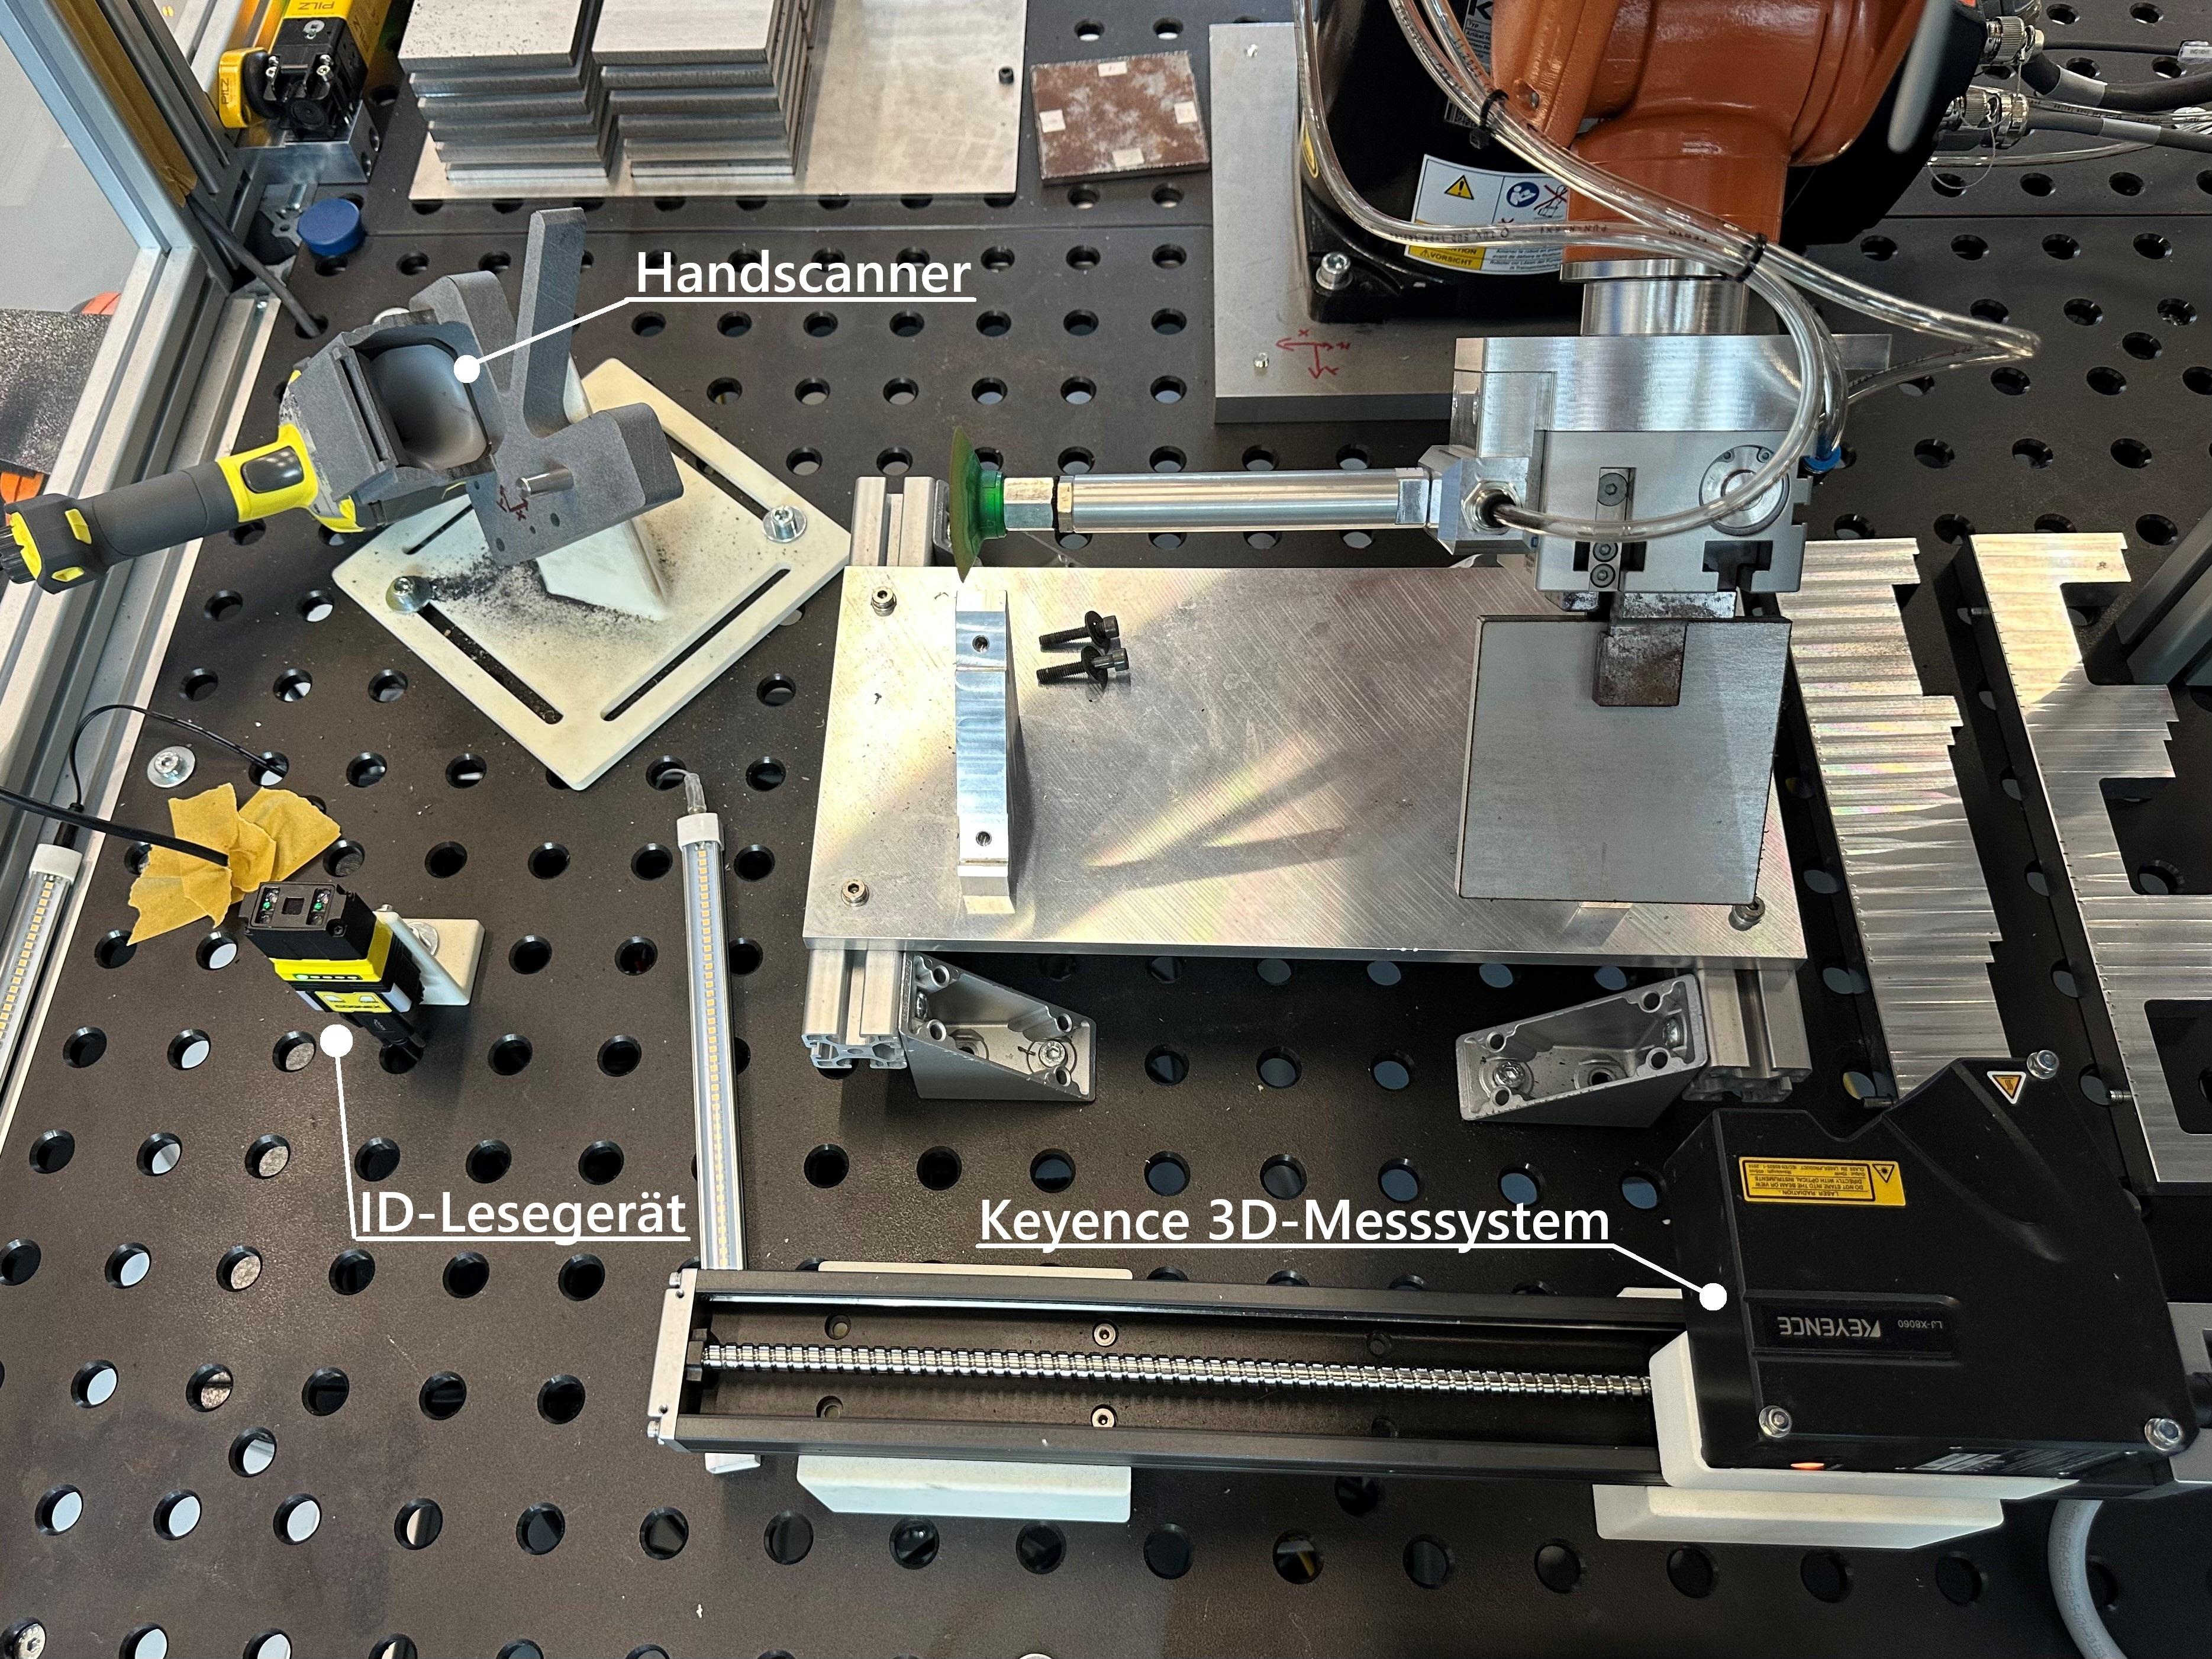
\includegraphics[width=0.7\linewidth]{handscanner_keyence.jpg}
    \caption{Handscanner (1), ID-Lesegerät (2), Keyence 3D-Messsystem (3) in der Messzelle}
    \label{fig:handscanner_barcodelesegerät_keyence}
\end{figure}

\newpage

Zur vollständigen Dokumentation werden die Schnittkanten zudem mit einer Industriekamera und einem stationären Smartphone-Setup unter verschiedenen Beleuchtungsbedingungen aufgenommen. Die Kombination aus unterschiedlichen Kameras und Beleuchtungen erhöht die Robustheit der visuellen Beurteilbarkeit und unterstützt die spätere manuelle Nachvollziehbarkeit von Auffälligkeiten. Die erfassten Messdaten des Werkstücks, sowie die daraus abgeleiteten Kenngrößen der Proben-ID zugeordnet und in die zentrale Datenbank überführt.

\begin{figure}[htbp]
    \centering
    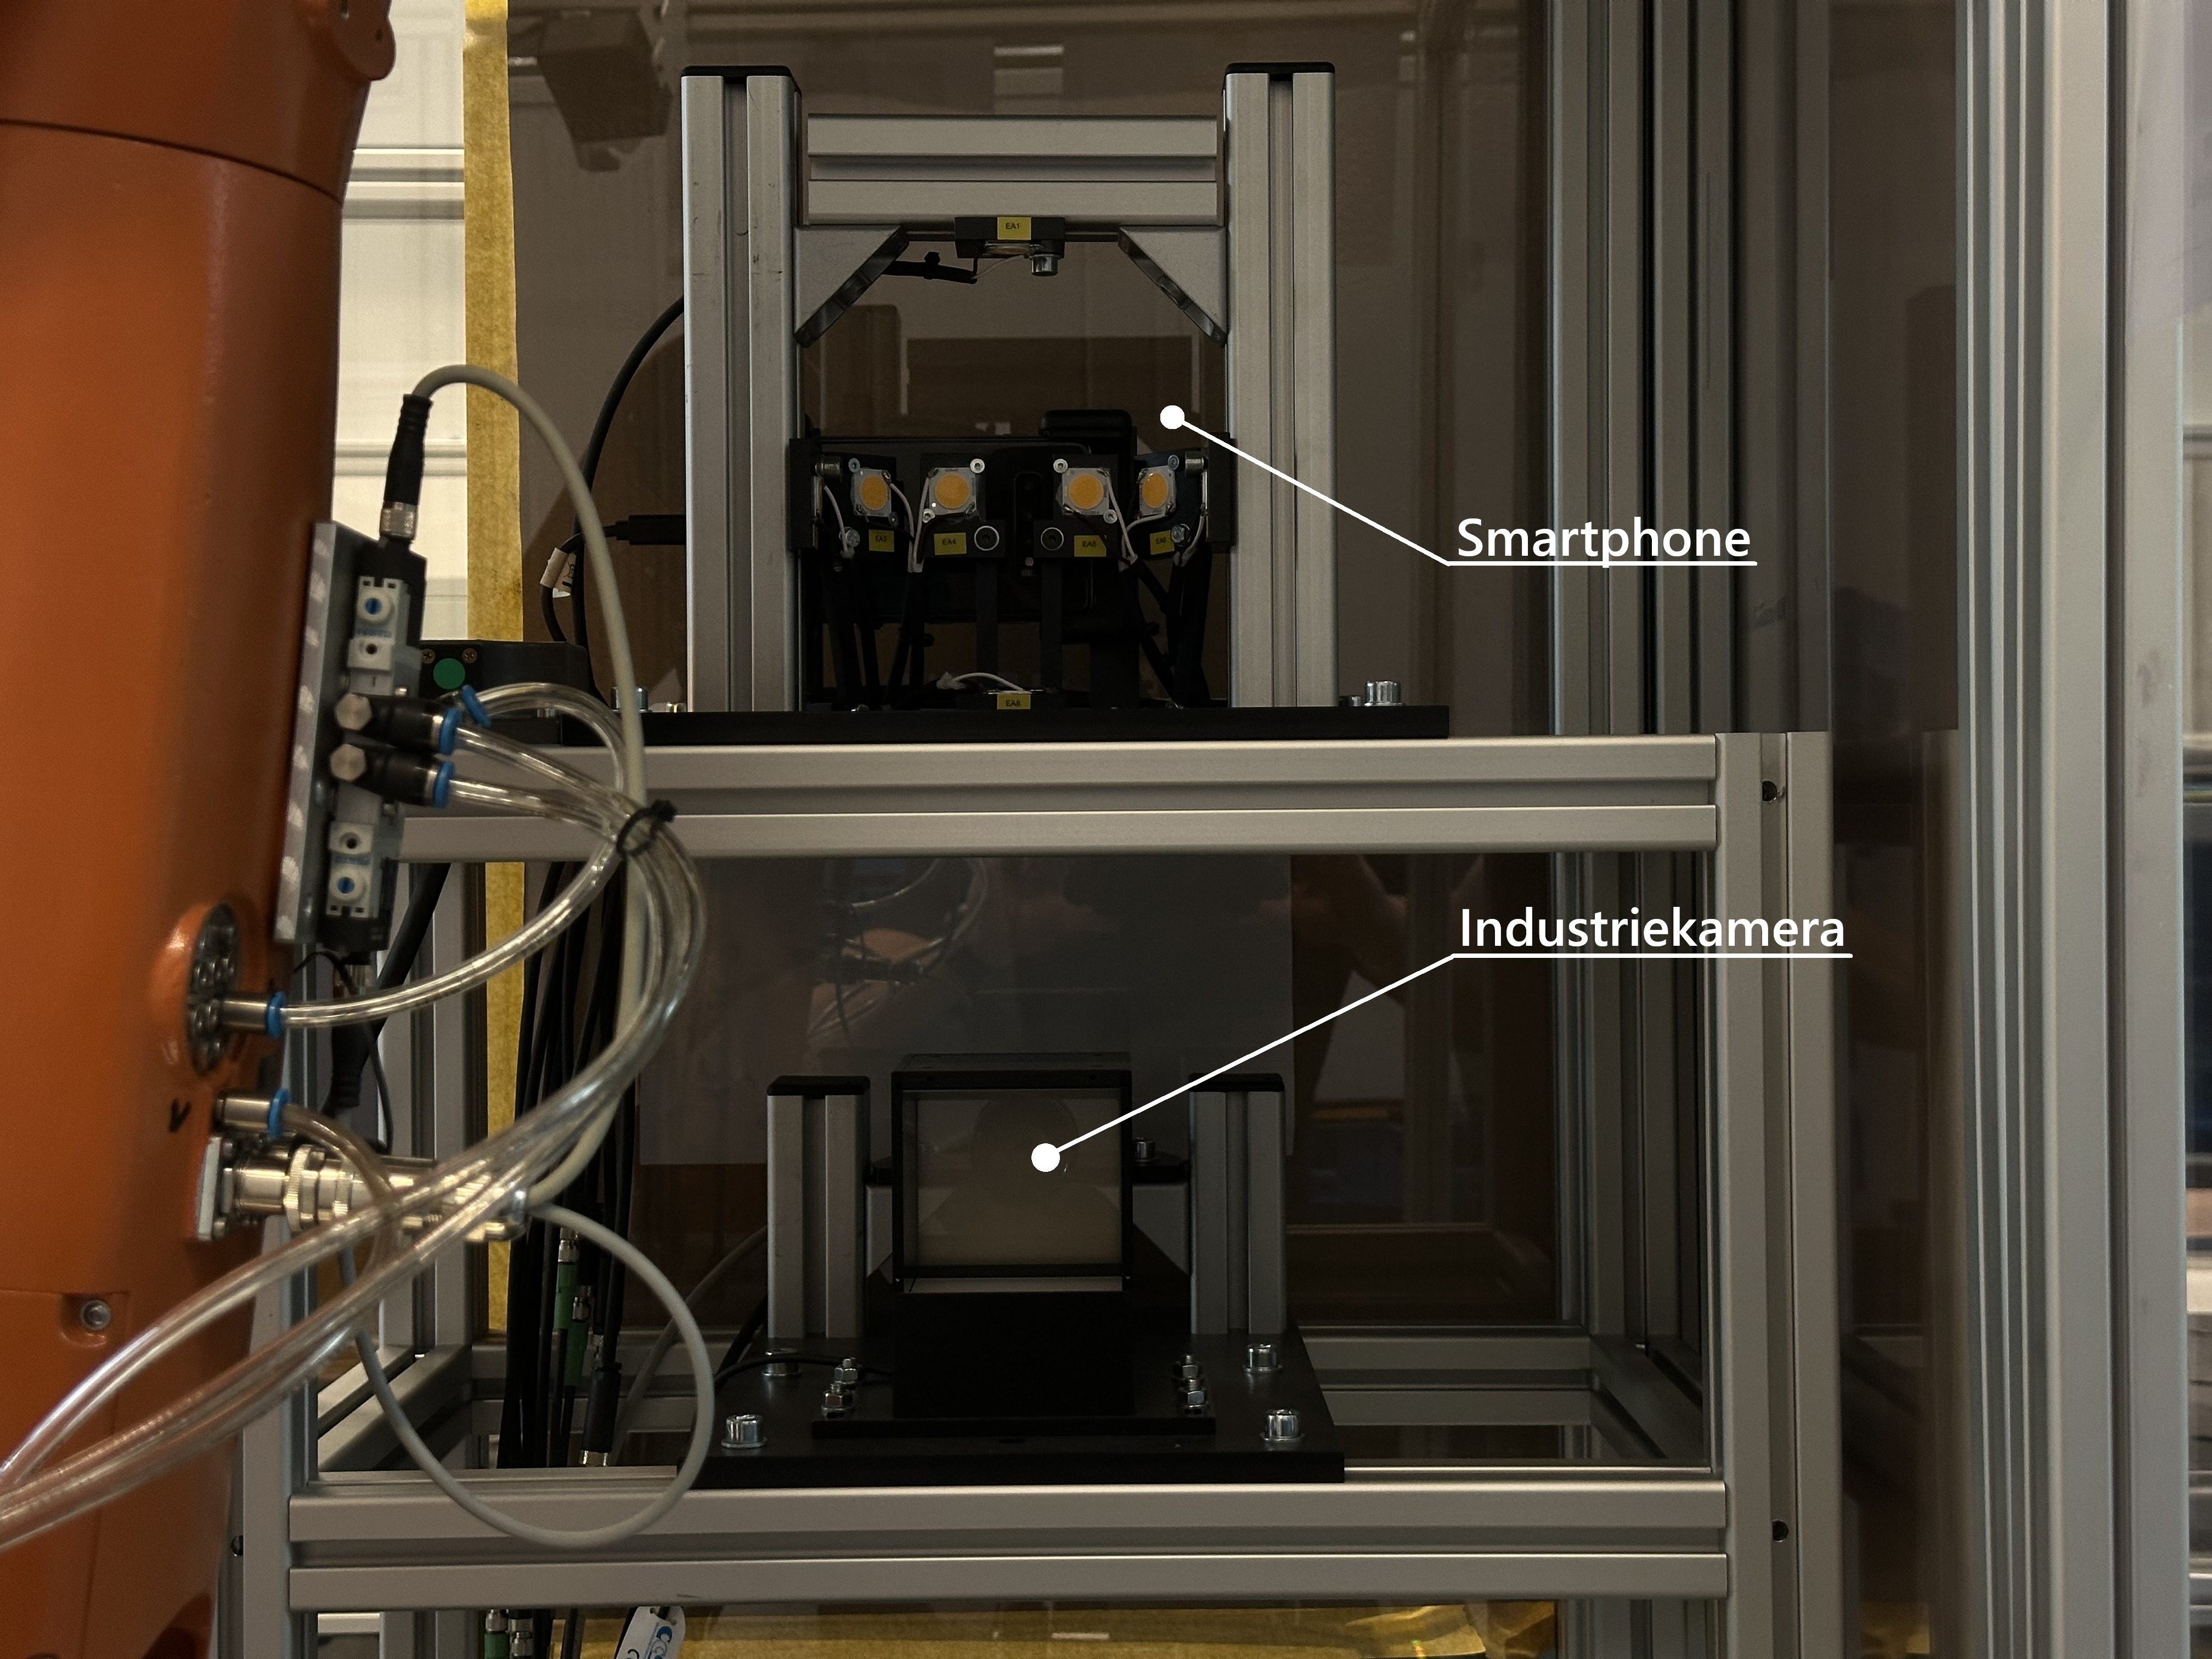
\includegraphics[width=0.7\linewidth]{smartphone_industriekamera.jpg}
    \caption{Smartphone (4) und Industriekamera (5) in der Messzelle}
    \label{fig:smartphone_industriekamera}
\end{figure}

Nach der Datenerfassung werden aus der 3D-Messung die tatsächlichen Kenngrößen der Schnittkante berechnet und den Ergebnissen der bildbasierten Qualitätsschätzung gegenübergestellt. Dieser Abgleich ermöglicht die Beurteilung der Übereinstimmung zwischen qualitativer, bildgestützter Bewertung und quantitativer Geometriemessung. Die beschriebenen Messschritte werden für alle vier Schnittkanten jedes Bauteils identisch wiederholt. Abschließend legt der Roboter die vollständig vermessenen Proben an der Endstation geordnet ab.

\newpage

\section{Anpassung des Handscanner-Setups}

Für die bildgestützte Qualitätsschätzung werden die mit dem Handscanner aufgenommenen Schnittkantenbilder als zentrale Eingangsgröße verwendet. Die bisher im Einsatz befindlichen Aufnahmeparameter waren für Baustahl optimiert. Baustahl weist im Vergleich zu Edelstahl eine geringere Oberflächenreflexion und eine tendenziell matte Erscheinung auf. Werden diese Einstellungen unverändert auf Edelstahl angewandt, führt die höhere Reflexion zu Bildartefakten und zu einer unzureichenden Abbildung der relevanten Mikrostruktur. In der Folge würden Grate (\emph{engl. Burr}) unterrepräsentiert und die Rauheit (\emph{engl. Roughness}) potenziell verfälscht erscheinen. Da die Klassifikation der Bildqualität und die darauf basierende Schätzung von \emph{Burr} und \emph{Roughness} unmittelbar in die Parametrierung des Laserschneidprozesses zurückwirken, ist eine werkstoffabhängige Anpassung des Handscanner-Setups zwingend erforderlich.

Das Aufnahmeprotokoll sieht pro Schnittkante drei Bilder vor: (i) ein bewusst dunkler belichtetes Bild, das primär der Beurteilung der Schnittflächenrauheit dient, sowie (ii) zwei überbelichtete Bilder, die gemeinsam mit dem ersten zu einem HDR-Komposit zusammengeführt werden, um die Kontur und Ausprägung des Grats sicher zu erfassen. Die Kalibrierung der Belichtung erfolgt schrittweise. Zunächst wird die Belichtungszeit für das Rauheitsbild so eingestellt, dass die Textur der Schnittfläche ohne Sättigung und mit klarer Detailzeichnung sichtbar ist. Diese Entscheidung erfolgt in dieser Phase bewusst subjektiv, jedoch anhand vorab definierter visueller Kriterien, wie z.B. ausreichender Tonwertumfang und erkennbarer Strukturkontrast. Im Anschluss werden die Belichtungsparameter der beiden HDR-Bilder iterativ variiert, bis der Grat entlang der Schnittkante über den gesamten Bildbereich eindeutig detektierbar ist, ohne dass umliegende Bereiche vollständig verloren gehen. Da die HDR-Komposition durch die Eingangsbilder beeinflusst wird, erfolgt die Abstimmung der HDR-Belichtungen stets nach der Festlegung des Rauheitsbildes. 
Die Abbildungen~\ref{fig:burr_baustahl},~\ref{fig:burr_edelstahl}, ~\ref{fig:roughness_baustahl} und ~\ref{fig:roughness_edelstahl} zeigen exemplarisch die finalen Handscanner Bilder, welche für die Qualitätsschätzung genutzt werden, für Edelstahl im Vergleich zu den bisherigen Bildern für die Qualitätsschätzung von Baustahl. In den Abbildungen ist jeweils die gleiche Schnittkante eines Blechteils aus den geschnittenen Experimentalplänen dargestellt mit einer Dicke von 15 mm.

\begin{figure}[htbp]
  \centering
  \begin{minipage}{0.48\linewidth}
    \centering
    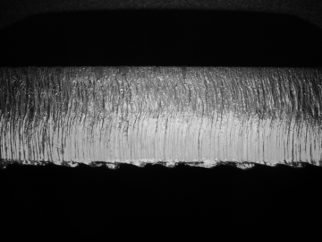
\includegraphics[width=\linewidth]{burr_baustahl.png}
    \caption{Handcanner Bild für die Gratschätzung (Baustahl)}
    \label{fig:burr_baustahl}
  \end{minipage}\hfill
  \begin{minipage}{0.48\linewidth}
    \centering
    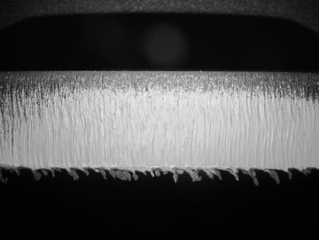
\includegraphics[width=\linewidth]{burr_edelstahl.png}
    \caption{Handcanner Bild für die Gratschätzung (Edelstahl)}
    \label{fig:burr_edelstahl}
  \end{minipage}
\end{figure}

\begin{figure}[htbp]
  \centering
  \begin{minipage}{0.48\linewidth}
    \centering
    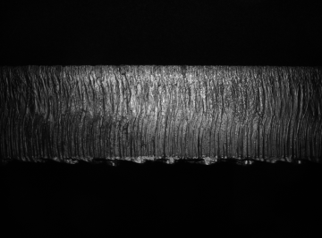
\includegraphics[width=\linewidth]{roughness_baustahl.png}
    \caption{Handscnanner Bild für die Rauheitsschätzung (Baustahl)}
    \label{fig:roughness_baustahl}
  \end{minipage}\hfill
  \begin{minipage}{0.48\linewidth}
    \centering
    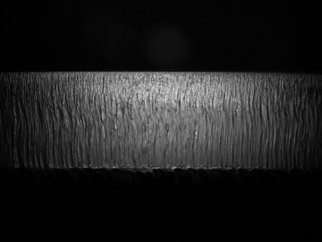
\includegraphics[width=\linewidth]{roughness_edelstahl.png}
    \caption{Handscanner Bild für die Rauheitsschätzung (Edelstahl)}
    \label{fig:roughness_edelstahl}
  \end{minipage}
\end{figure}

Zur Sicherstellung der Kompatibilität mit dem bestehenden KI-Modell wird die Anpassung an Referenzaufnahmen aus der bereits validierten Baustahlkonfiguration ausgerichtet. Praktisch bedeutet dies, dass eine Baustahlschnittkante mit den etablierten Baustahleinstellungen aufgenommen wird und die Edelstahlaufnahmen so justiert werden, dass die resultierenden Bildcharakteristika in qualitativer Hinsicht vergleichbar sind. Auf diese Weise wird gewährleistet, dass die Edelstahlbilder in das bestehende Modell eingebunden und mit den vorhandenen Trainings- und Bewertungsroutinen verarbeitet werden können.

Zur konsistenten Anwendung der angepassten Handscanner-Parameter wird das Messzellen-Skript so erweitert, dass das passende Setup automatisiert auf Basis der Bauteilbezeichnung gewählt wird. Die Benennung folgt dem Schema
\texttt{Maschinenname-\allowbreak Experimentalplanname-\allowbreak Materia
lnummer-\allowbreak Bauteildicke-\allowbreak Bauteilnummer},
z.\,B.\ \texttt{A02280E0005-\allowbreak AiMuWrCjd0-\allowbreak 3-\allowbreak 050-\allowbreak 0176}.
Die folgende Abbildung ~\ref{fig:probenID} zeigt eine Beispiel-Proben-ID eines Blechstücks aus den Experimentalplänen mit den einzelnen Segmenten.

\begin{figure}[htbp]
    \centering
    \includegraphics[width=0.7\linewidth]{Werkstück_Proben-ID.jpg}
    \caption{Beispiel-Proben-ID eines Blechstücks aus den Experimentalplänen}
    \label{fig:probenID}
\end{figure}

Das Skript parst die Zeichenkette, prüft die Zahl nach dem zweiten Bindestrich und lädt abhängig davon die vordefinierten Handscanner-Einstellungen für den jeweiligen Werkstoff. Auf diese Weise wird sichergestellt, dass die für Edelstahl kalibrierten Belichtungen und Aufnahmeparameter reproduzierbar zur Anwendung kommen und die so erzeugten Bilder ohne systematische Verzerrungen in die Qualitätsmodellierung eingehen. Dies ist im folgendem C-Sharp Quellcode ~\ref{lst:messzellen-routing} dargestellt und im Messzellenskript inplementiert.

\begin{lstlisting}[language={[Sharp]C}, caption={Werkstoffabhängiges Routing der Handscanner-Setups}, label={lst:messzellen-routing}]
public static string NameParserMaterial(string input)
{
    if (string.IsNullOrWhiteSpace(input))
        return "ST";                                // Fallback-Wert

    // Position des ersten und zweiten Bindestrichs ermitteln
    int firstDash = input.IndexOf('-');
    int secondDash = firstDash >= 0
                   ? input.IndexOf('-', firstDash + 1)
                   : -1;

    // Prüfen, ob ein zweiter Bindestrich und ein Zeichen dahinter existieren
    if (secondDash < 0 || secondDash + 1 >= input.Length)
        return "ST";                                // Fallback-Wert

    char digit = input[secondDash + 1];             // Ziffer einlesen

    // Zuordnung: 1 → "ST", 2 → "ST", 3 → "SS" (bei Bedarf anpassen)
    return digit switch
    {
        '1' => "ST",
        '2' => "ST",
        '3' => "SS",
        _ => "ST"                                   // Default
    };
}
\end{lstlisting}

\section{Optimierung der Vektorberechnung aus 3D-Punktwolken}

Die mit dem Keyence-System aufgenommene 3D-Punktwolke der Schnittkante bildet die Grundlage für die geometrische Qualitätsauswertung. In der bestehenden Auswertepipeline wird die Punktwolke zunächst segmentiert und in ein lokales Kantenkoordinatensystem überführt. Anschließend erfolgt eine Projektion aus der dreidimensionalen Repräsentation in einen zweidimensionalen Profilverlauf, sodass ein 2D-Vektor entsteht, der den Verlauf des Schneidgrats entlang der Schnittkante beschreibt. Diese Vorgehensweise wurde ursprünglich für Baustahl entwickelt und auf dessen charakteristisch eher wellige, kontinuierliche Gratmorphologie abgestimmt.

Die nachfolgend beschriebenen Anpassungen betreffen ausschließlich den \textbf{Grat-/Burr}-Kanal unterteilt in der Ausreißererkennung von Messdaten und der darauffolgenden Interpolation. Für die Rauheitsanalyse werden die in der Baustahl-Pipeline etablierten Einstellungen übernommen. Aus interner Erfahrung zeigt die Rauheitsprüfung eine stabile und konsistente bewertung, sodass in diesem Kapitel bewusst auf Abbildungen als Nachweis verzichtet wird.

Bei Edelstahl zeigt sich eine abweichende, ausgeprägt zackige Gratstruktur mit höheren lokalen Gradienten und diskontinuierlichen Profilabschnitten. Die bislang implementierte Outlier-Korrektur ist konzipiert zur Eliminierung sporadischer Messfehler bei Baustahl. Demnach stuft diese den Gratverlauf von Edelstahl fälschlich als Ausreißer ein und glättet sie übermäßig. Dadurch werden relevante Merkmale des Edelstahlgrats unterdrückt und der resultierende Vektorverlauf in Richtung eines künstlich „glatten“ Profils verzerrt.

Erschwerend kommt hinzu, dass im Messprozess partiell überbeschattete Bereiche auftreten können, die vom Sensor nicht erfasst werden. In der bisherigen Pipeline werden solche Lücken durch Interpolation geschlossen, deren Parameter auf die kontinuierlichen Profile von Baustahl zugeschnitten sind. Für den zackigen Edelstahlgrat führt dies zu einer zu starken Annäherung an glatte Zwischenverläufe und damit zu einem Verlust an formcharakteristischer Information.

Zur materialspezifischen Anpassung werden daher zwei Kernmodule überarbeitet. Die Ausreißererkennung \cref{sec:Outlier Detection/Correction} mit nachgelagerter Korrektur und die Interpolation \cref{sec:Interpolation} fehlender Stützstellen. In der Ausreißererkennung werden die Schwellwerte und die zugrunde liegenden Sensitivitätsmaße an die höhere lokale Krümmung und den gesteigerten Kantenkontrast des Edelstahlgrats angepasst. Ziel ist eine Differenzierung zwischen echten Messfehlern und materialtypischen Hochfrequenzanteilen. Entsprechend werden Glättungsschritte zurückgenommen, sodass signifikante Gratflanken erhalten bleiben. 

Für die Interpolation wird ein konservativer Ansatz gewählt, der Lückenschlüsse bevorzugt entlang lokal konsistenter Nachbarschaften vornimmt und globale, stark glättende Approximationen vermeidet. Damit wird erreicht, dass der rekonstruierte 2D-Vektor fehlende Messpunkte plausibel ergänzt, ohne die charakteristische Zackigkeit des Edelstahlgrats zu nivellieren.

\subsection{Outlier Detection/Correction}
\label{sec:Outlier Detection/Correction}

Die Ausreißerbehandlung im \textbf{Burr}-Kanal erfolgt zweistufig. Zunächst werden potenzielle Ausreißerpunkte durch den Vergleich des gemessenen Profils mit einem lokal geglätteten Referenzsignal identifiziert. Anschließend werden die dadurch entstehenden Lücken kontrolliert und rekonstruiert. In \texttt{outlier\_correction\_burr} wird das Höhenprofil \texttt{z\_vec} mittels gleitendem Mittelwert (\texttt{np.convolve} mit der Fensterlänge \texttt{window}) geglättet. Die absolute Abweichung \(\Delta=\lvert z-\overline{z}_{\text{MA}}\rvert\) wird punktweise gegen den Schwellwert \texttt{threshold} geprüft. Punkte oberhalb des Schwellwertes bilden die Ausreißermaske. Ist der Anteil markierter Punkte größer als \texttt{max\_nan\_values\_perc}, wird der Vorgang verworfen (\texttt{None}). Andernfalls werden die Ausreißer zu \texttt{NaN} gesetzt und mit \texttt{smooth\_nan\_values} rekonstruiert, um numerisches Rauschen zu reduzieren, ohne relevante Strukturen zu nivellieren.

Die Funktion \texttt{outlier\_correction\_profile\_lines} setzt denselben Ansatz für einzelne Profilzeilen um, verwendet jedoch standardmäßig einen robusten gleitenden Median (\texttt{median=True}) als Referenzsignal. Aus der Abweichung zum Referenzsignal wird eine Ausreißermaske gebildet und über \texttt{max\_outlier\_values\_perc} validiert. Markierte Punkte werden zu \texttt{NaN} gesetzt und anschließend nur dann interpoliert, wenn die Lückenlänge die Vorgabe \texttt{max\_gap} nicht überschreitet (\texttt{interpolate\_limited\_nans}).Die Rauheitsanalyse nutzt unverändert die etablierten Baustahl-Einstellungen, hierfür erfolgt keine Umparametrisierung.

\begin{lstlisting}[language=Python, caption={Outlier Detection/Correction in der Profilvorverarbeitung (Burr-Kanal)}, label={lst:outlier-correction}]
def outlier_correction_burr(x_vec, z_vec, threshold=0.04, window=20, max_nan_values_perc=0.4):
    """
    Entfernt Ausreißer anhand eines Moving-Average-Vergleichs.
    """
    z_vec = np.copy(z_vec)
    z_smoothed = np.convolve(z_vec, np.ones(window) / window, mode='same')
    difference = np.abs(z_vec - z_smoothed)

    outlier_mask = difference > threshold
    num_outliers = np.sum(outlier_mask)

    if num_outliers / len(z_vec) > max_nan_values_perc:
        return None, None

    z_vec[outlier_mask] = np.nan
    z_vec_clean = smooth_nan_values(x_vec, z_vec)

    return x_vec, z_vec_clean


def outlier_correction_profile_lines(line, outlier_threshold=0.04, window_size=30,
                                     median=True, max_outlier_values_perc=0.35, max_gap=5):
    """
    Entfernt Ausreißer in Höhenprofilen basierend auf Median- oder Mittelwert-Vergleich.
    """
    Z_series = pd.Series(line)
    tmp_line = line.copy()

    if median:
        moving_avg = Z_series.rolling(window_size, min_periods=5, center=True).median()
    else:
        moving_avg = Z_series.rolling(window_size, min_periods=5, center=True).mean()

    difference = np.abs(line - moving_avg)
    id_outlier = difference > outlier_threshold
    count_outlier = np.sum(id_outlier)

    if count_outlier / len(line) > max_outlier_values_perc:
        return None, None

    tmp_line[id_outlier] = np.nan
    tmp_line = interpolate_limited_nans(tmp_line, max_gap=max_gap)

    return tmp_line, moving_avg
\end{lstlisting}

In der Edelstahl-Pipeline wurden die Schwellwerte der Burr-Outlier-Korrektur angehoben und das Fenster leicht verkürzt, um zackige, materialspezifische Hochfrequenzanteile nicht fälschlich als Ausreißer zu markieren. Zum Vergleich sind nachfolgend die verwendeten Parameter für Edelstahl sowie die bisherige Baustahl-Konfiguration aufgeführt (siehe auch Quellcode~\ref{lst:params-outlier-stainless} und Quellcode~\ref{lst:params-outlier-mild}). Für die Rauheitsanalyse wurden keine Parameteränderungen vorgenommen.

\begin{lstlisting}[caption={Pipeline-Parameter Outlier Correction (Edelstahl, Burr-Kanal)}, label={lst:params-outlier-stainless}]
# Parameter burr outlier correction (Edelstahl)
burr_outlier_threshold : 0.06  # Threshold for Moving Average Difference Filter [mm]
burr_outlier_window    : 9     # Window for Moving Average Difference Filter [samples]
\end{lstlisting}

\begin{lstlisting}[caption={Pipeline-Parameter Outlier Correction (Baustahl, Burr-Kanal)}, label={lst:params-outlier-mild}]
# Parameter burr outlier correction (Baustahl)
burr_outlier_threshold : 0.03  # Threshold for Moving Average Difference Filter [mm]
burr_outlier_window    : 10    # Window for Moving Average Difference Filter [samples]
\end{lstlisting}

\subsection{Interpolation}
\label{sec:Interpolation}

Die Interpolation dient der Rekonstruktion fehlender Messwerte (\texttt{NaN}), die durch Ausreißererkennung oder unvollständige Erfassung entstehen. Ziel ist eine Wiederherstellung des Gratverlaufs, demnach werden nur kurze, lokal begrenzte Lücken gefüllt und größere Ausfälle bleiben aus. Der Rekonstruktionsschritt nutzt ausschließlich lokale Nachbarschaftsinformationen, um die charakteristische Profil- bzw.\ Kantenstruktur zu erhalten und unnötige Verfälschungen zu vermeiden.

In der Interpolations-Pipeline wurden keine Konstanten geändert. Insbesondere bleiben Grenzwerte für die maximale Lückenlänge sowie Glättungs- und Fensterparameter gegenüber der Baustahlkonfiguration unverändert. Der zugehörige Quellcode ist im Anhang dokumentiert.

\section {Validierung der Messoptimierungen}